% !TeX root = ../main.tex
\section{Luật Chơi Qua Hình Ảnh}
\label{sec:rules}

Đây là phần chính trình bày luật chơi bằng \emph{ảnh chụp trực tiếp từ
trò chơi} thay cho công thức, đủ để người đọc không chuyên toán nắm được
toàn bộ trò chơi; đặc tả toán học hình thức tương ứng (chế độ 2 người) nằm
ở Phụ lục~\ref{app:formal}. Quy ước: quân \textbf{Xanh} tô xanh lá, quân
\textbf{Vàng} tô vàng; quân \emph{đỉnh} nằm trên giao điểm lưới ô vuông,
quân \emph{tâm} nằm giữa bốn đỉnh. Các chỉ dấu trong ảnh đều do chính trò
chơi vẽ: \emph{vòng vàng} đánh dấu quân đang được chọn, \emph{chấm xanh}
là ô đáp hợp lệ, và \emph{đường vàng} chỉ hướng ăn (sandwich) từ ô đáp.

\subsection{Bàn cờ---41 ô trên hai lớp}
\label{ssec:vis_board}

\begin{figure}[H]
  \centering
  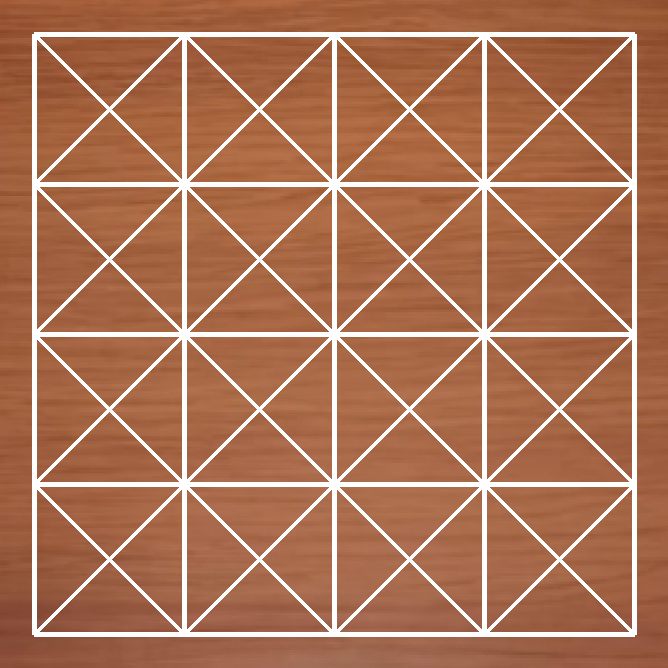
\includegraphics[width=0.5\linewidth]{figures/board_2p_empty.png}
  \caption{Cấu trúc bàn cờ chế độ 2 người (ảnh chụp trực tiếp từ trò chơi):
  25 ô \textbf{đỉnh} (giao điểm của lưới ô vuông, toạ độ nguyên như
  $(0,0),(2,3)$) cộng 16 ô \textbf{tâm} (giao điểm các đường chéo, nửa
  nguyên như $(0.5,0.5)$), mỗi ô tâm nằm chính giữa bốn ô đỉnh. Tổng 41 ô.
  Quân đỉnh và quân tâm hoạt động trên hai lớp riêng nhưng đan nhau qua
  đường chéo.}
  \label{fig:board41}
\end{figure}

\begin{table}[H]
  \centering
  \caption{Kích thước bàn cờ và cấu hình theo chế độ chơi (toạ độ và vị trí
  xuất phát chính xác cho 3--4 người ở Phụ lục~\ref{app:multistart}).}
  \label{tab:board_size}
  \begin{tabular}{lcccc}
    \toprule
    \textbf{Chế độ} & \textbf{Kích thước} & \textbf{Toạ độ}
    & \textbf{Ô bị loại} & \textbf{Quân/người} \\
    \midrule
    2 người & 5{\texttimes}5 đỉnh & $0\text{--}4 \times 0\text{--}4$ & 0 & 14 \\
    3 người & 7{\texttimes}6 đỉnh & $0\text{--}6 \times 0\text{--}5$ & 4 & 13/13/14 \\
    4 người & 7{\texttimes}7 đỉnh & $0\text{--}6 \times 0\text{--}6$ & 8 & 13 \\
    \bottomrule
  \end{tabular}
\end{table}

\subsection{Vị trí xuất phát---trạng thái 0}
\label{ssec:vis_start}

\begin{figure}[H]
  \centering
  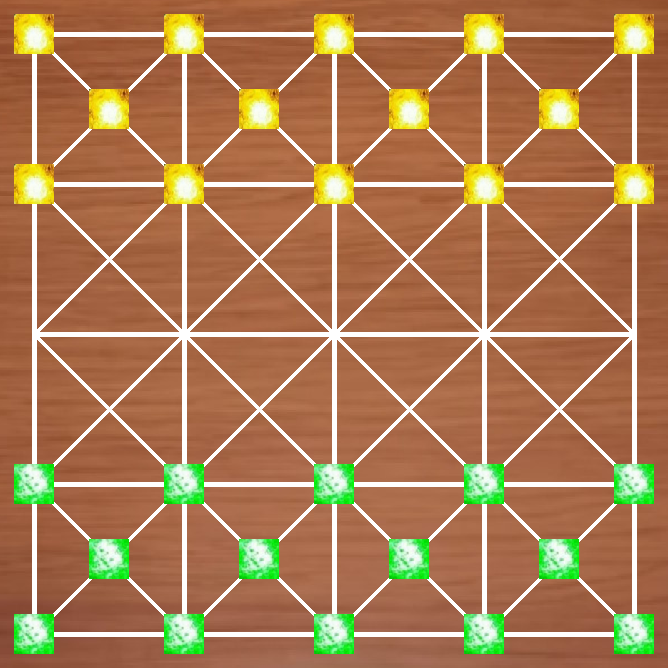
\includegraphics[width=0.5\linewidth]{figures/board_2p.png}
  \caption{28 quân ở vị trí xuất phát (ảnh chụp trực tiếp từ trò chơi):
  Vàng và Xanh lá, mỗi phe 14 quân ($=10$ đỉnh $+\,4$ tâm) chiếm hai hàng
  ở hai phía đối diện của bàn; ba hàng giữa để trống. Đối chiếu công
  thức~\eqref{eq:starty}--\eqref{eq:startg}.}
  \label{fig:start}
\end{figure}

\subsection{Hướng đi---quân di chuyển theo hướng nào}
\label{ssec:vis_dirs}

\begin{figure}[H]
  \centering
  \begin{subfigure}[b]{0.46\linewidth}\centering
    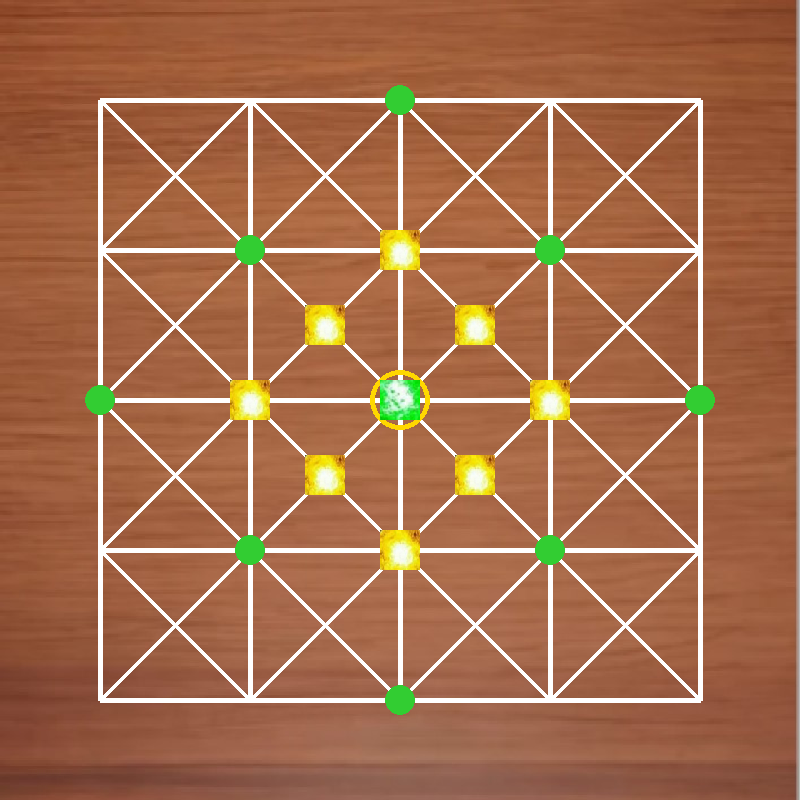
\includegraphics[height=3.4cm]{figures/dir_vertex.png}
    \caption{Quân \textbf{đỉnh}---8 hướng: 4 ngang--dọc (bước 1, qua ô
    đỉnh kề) $+$ 4 chéo (bước $\tfrac12$, qua ô tâm).}
  \end{subfigure}\hfill
  \begin{subfigure}[b]{0.46\linewidth}\centering
    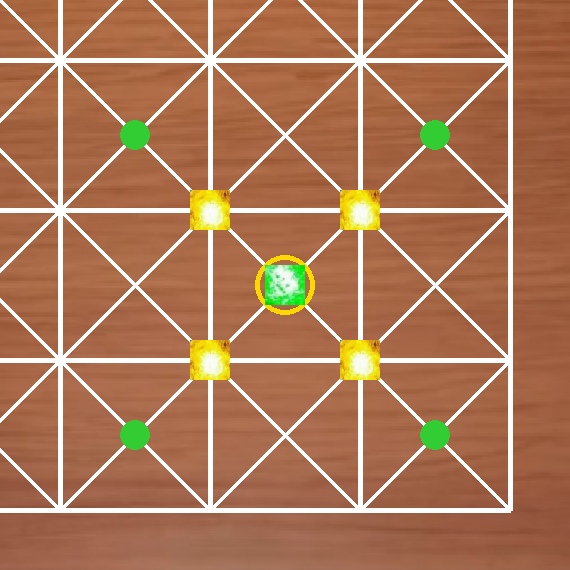
\includegraphics[height=3.4cm]{figures/dir_center.png}
    \caption{Quân \textbf{tâm}---chỉ 4 hướng chéo (mỗi bước qua một ô
    đỉnh kề). Đi ngang--dọc sẽ rơi khỏi lớp tâm.}
  \end{subfigure}
  \caption{Các hướng đi (ảnh từ trò chơi; quân được chọn có vòng vàng, các
  \emph{chấm xanh} là ô đáp hợp lệ do trò chơi tô sẵn), tương ứng tập
  $D_{\mathsf V}$ và $D_{\mathsf C}$ ở~\eqref{eq:dirs}.}
  \label{fig:dirs}
\end{figure}

\subsection{Cú nhảy---cách di chuyển duy nhất}
\label{ssec:vis_jump}

Quân \emph{chỉ} di chuyển bằng cách nhảy: bay qua một ô kề có quân làm
\emph{bệ} (phe nào cũng được) và đáp xuống ô trống ngay sau đó; quân làm
bệ đứng nguyên. Hình~\ref{fig:jumps} minh hoạ ba loại nhảy.

\begin{figure}[H]
  \centering
  % Ví dụ 1: đỉnh nhảy ngang
  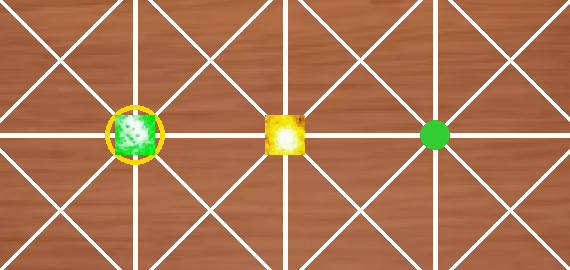
\includegraphics[height=1.9cm]{figures/jump1_before.png}\;$\rightarrow$\;%
  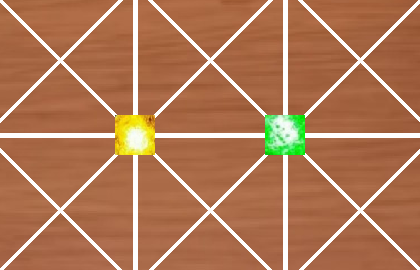
\includegraphics[height=1.9cm]{figures/jump1_after.png}
  \\[0.6em]
  % Ví dụ 2: đỉnh nhảy chéo
  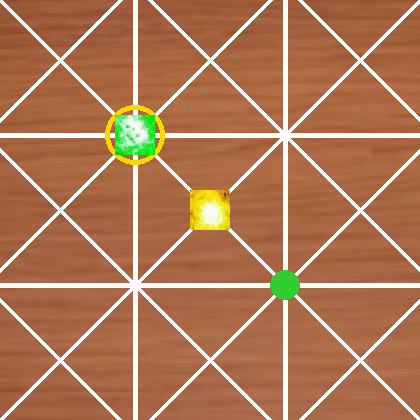
\includegraphics[height=2.3cm]{figures/jump2_before.png}\;$\rightarrow$\;%
  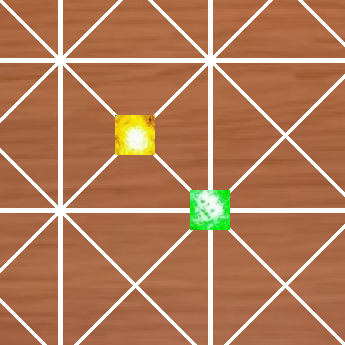
\includegraphics[height=2.3cm]{figures/jump2_after.png}
  \\[0.6em]
  % Ví dụ 3: tâm nhảy chéo
  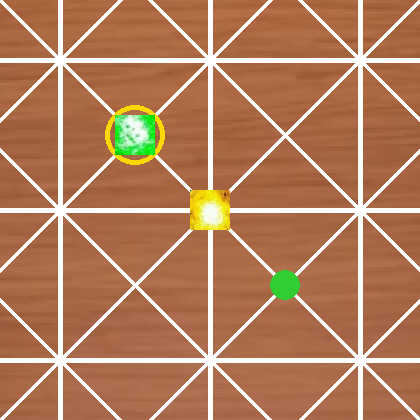
\includegraphics[height=2.3cm]{figures/jump3_before.png}\;$\rightarrow$\;%
  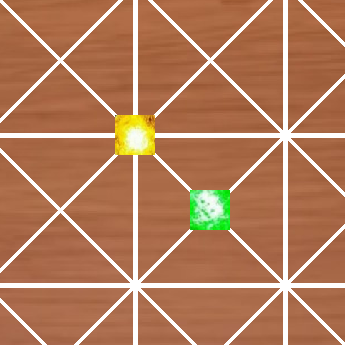
\includegraphics[height=2.3cm]{figures/jump3_after.png}
  \caption{Ba ví dụ nhảy (ảnh từ trò chơi, trước $\rightarrow$ sau; vòng
  vàng = quân được chọn, chấm xanh = ô đáp hợp lệ). \textbf{Trên:} quân
  đỉnh nhảy ngang qua bệ $(2,2)$, đáp $(3,2)$. \textbf{Giữa:} quân đỉnh
  nhảy chéo dùng ô \emph{tâm} $(1.5,1.5)$ làm bệ, đáp ô đỉnh $(2,2)$.
  \textbf{Dưới:} quân tâm nhảy chéo dùng ô \emph{đỉnh} $(2,2)$ làm bệ,
  đáp ô tâm $(2.5,2.5)$. Bệ nhảy luôn ở nguyên chỗ, không đổi phe.}
  \label{fig:jumps}
\end{figure}

\subsection{Cách bắt quân---kẹp và lật}
\label{ssec:vis_capture}

\emph{Đáp xuống đâu, nhìn quanh đó}: từ ô đáp, theo từng hướng, một dãy
quân địch liền nhau mà ngay sau là một quân mình thì bị kẹp và đổi phe.
Hình~\ref{fig:capture} cho một tình huống có \emph{hai} hướng ăn được;
Bảng~\ref{tab:capture_rays} liệt kê chi tiết.

\begin{figure}[H]
  \centering
  \begin{subfigure}[b]{0.42\linewidth}\centering
    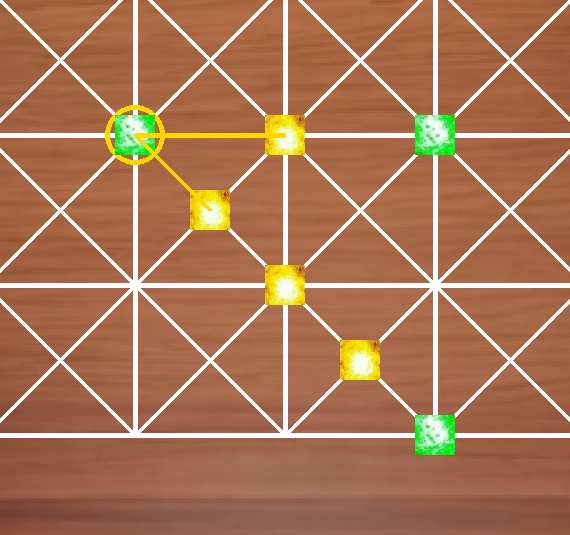
\includegraphics[height=4cm]{figures/capture_before.png}
    \caption{Vừa đáp $(1,2)$: trò chơi tô \emph{hai} tia ăn được (vàng).}
  \end{subfigure}\hfill
  \begin{subfigure}[b]{0.42\linewidth}\centering
    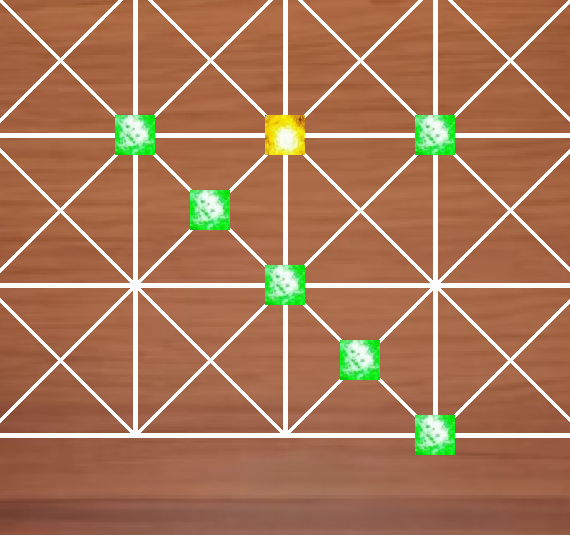
\includegraphics[height=4cm]{figures/capture_after.png}
    \caption{Sau khi chọn tia chéo và lật (3 quân).}
  \end{subfigure}
  \caption{Quân Xanh vừa đáp $(1,2)$ (ảnh từ trò chơi). Có hai hướng ăn
  được; người đi chọn \emph{một}. Chọn tia chéo: ba quân Vàng
  $(1.5,2.5),(2,3),(2.5,3.5)$ đổi thành Xanh, còn $Y@(2,2)$ của tia ngang
  \emph{vẫn Vàng}---hướng không chọn thì không lật.}
  \label{fig:capture}
\end{figure}

\begin{table}[H]
  \centering
  \caption{Hai hướng ăn được từ ô đáp $(1,2)$ trong Hình~\ref{fig:capture}.}
  \label{tab:capture_rays}
  \begin{tabular}{lll}
    \toprule
    \textbf{Hướng} & \textbf{Tia chạy qua} & \textbf{Số quân kẹp} \\
    \midrule
    Ngang $(1,0)$ & $(2,2){=}\mathrm Y \to (3,2){=}\mathrm G$ & \textbf{1} \\
    Chéo $(\tfrac12,\tfrac12)$
      & $(1.5,2.5){=}\mathrm y \to (2,3){=}\mathrm Y \to (2.5,3.5){=}\mathrm y \to (3,4){=}\mathrm G$
      & \textbf{3} (2 tâm $+$ 1 đỉnh) \\
    Hướng khác & đứt mạch (gặp ô trống hoặc ra biên) & 0 \\
    \bottomrule
  \end{tabular}
\end{table}

\noindent\textbf{Luật chọn:} có kẹp thì \emph{phải} ăn, và chọn đúng
\emph{một} hướng. Chính sách ``luôn chọn hướng ăn nhiều nhất'' mà bot hay
dùng chỉ là chiến thuật, không phải luật---người chơi có quyền ăn ít hơn
để giăng bẫy.

\subsection{Một nước đi diễn ra thế nào---ba bước}
\label{ssec:vis_move}

\begin{figure}[H]
  \centering
  \begin{subfigure}[b]{0.32\linewidth}\centering
    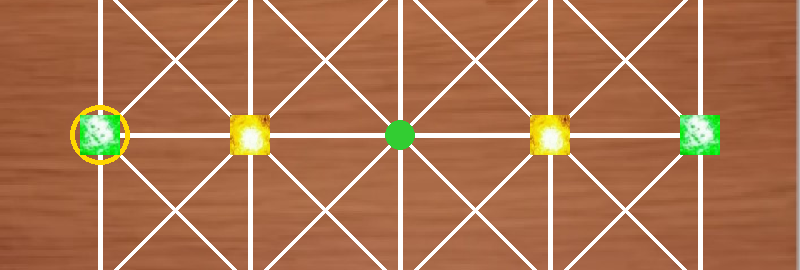
\includegraphics[width=\linewidth]{figures/move_a.png}
    \caption{A. Trước nhảy.}
  \end{subfigure}\hfill
  \begin{subfigure}[b]{0.32\linewidth}\centering
    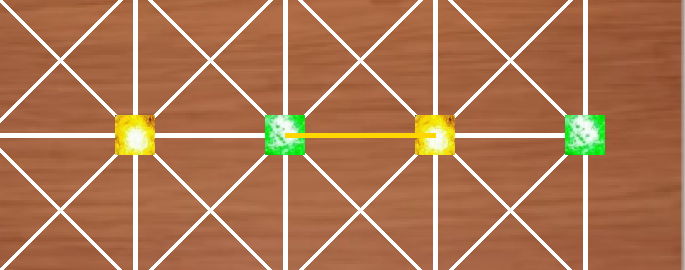
\includegraphics[width=\linewidth]{figures/move_b.png}
    \caption{B. Sau nhảy, chưa lật.}
  \end{subfigure}\hfill
  \begin{subfigure}[b]{0.32\linewidth}\centering
    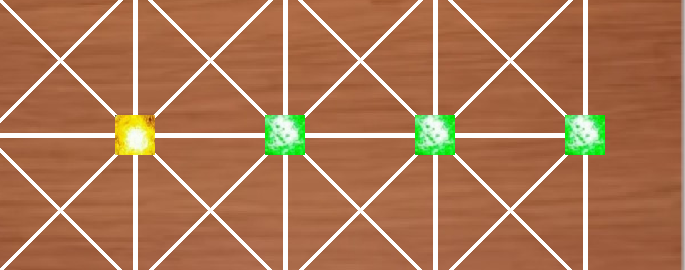
\includegraphics[width=\linewidth]{figures/move_c.png}
    \caption{C. Sau lật, đổi lượt.}
  \end{subfigure}
  \caption{Một nước đi đầy đủ (ảnh từ trò chơi). (A) $G@(0,2)$ nhảy qua bệ $Y@(1,2)$, đáp
  $(2,2)$. (B) tia phải phát hiện kẹp $Y@(3,2)$ giữa quân mới và $G@(4,2)$.
  (C) $Y@(3,2)$ đổi sang Xanh; bệ nhảy $Y@(1,2)$ \emph{vẫn Vàng}; đến lượt
  Vàng. Ba bước ứng với~\eqref{eq:t1}--\eqref{eq:t3}.}
  \label{fig:fullmove}
\end{figure}

\subsection{Khi nào ván kết thúc}
\label{ssec:vis_end}

Đến lượt phe nào mà phe đó không còn quân nào nhảy được thì thua ngay
(điều kiện~\eqref{eq:terminal}). Có hai kiểu thua, Hình~\ref{fig:endgame}.

\begin{figure}[H]
  \centering
  \begin{subfigure}[b]{0.46\linewidth}\centering
    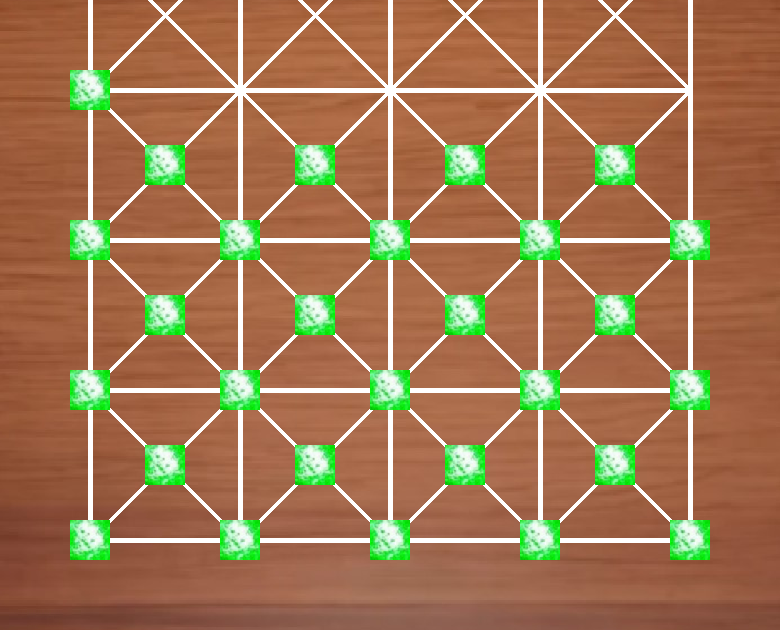
\includegraphics[height=4.2cm]{figures/end_nopieces.png}
    \caption{Hết quân: cả 28 quân đã thuộc Xanh, Vàng không còn gì để đi.}
  \end{subfigure}\hfill
  \begin{subfigure}[b]{0.46\linewidth}\centering
    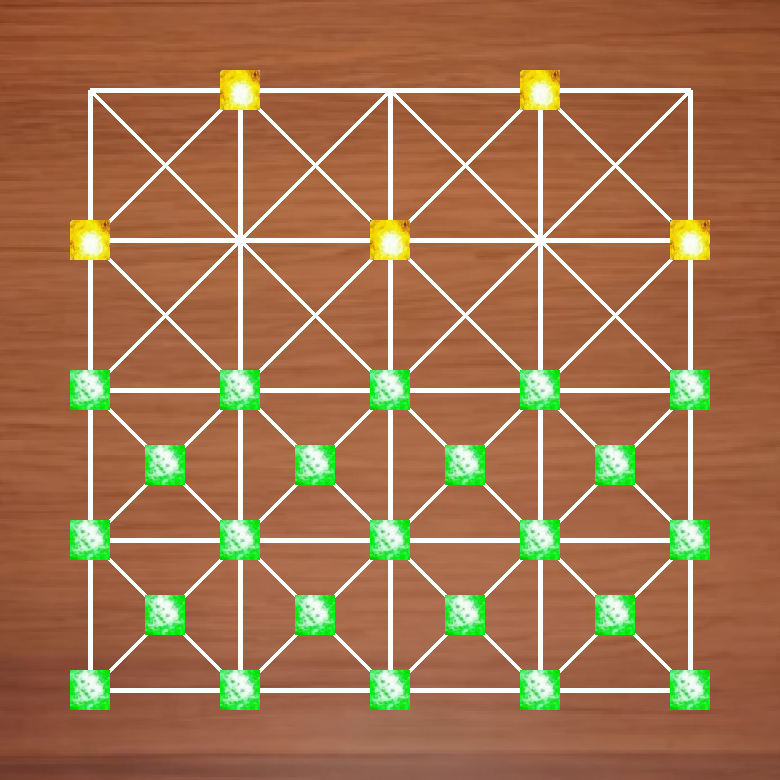
\includegraphics[height=4.2cm]{figures/end_blocked.png}
    \caption{Bị phong toả: Vàng còn 5 quân nhưng mọi ô đáp đều bị chiếm
    hoặc ra ngoài bàn (ví dụ rút gọn).}
  \end{subfigure}
  \caption{Hai cách thua. Chế độ 2 người không có hoà. Phe tạm hết nước
  khi \emph{chưa} tới lượt mình thì chưa thua---chỉ xét đúng đầu lượt.}
  \label{fig:endgame}
\end{figure}
